\documentclass[manuscript,screen,review,nonacm]{acmart}
\usepackage{graphicx}
\usepackage{hyperref}
\usepackage[
backend=biber,
style=alphabetic,
sorting=ynt
]{biblatex}
\addbibresource{bibliography.bib}



\setcopyright{none}
\settopmatter{printacmref=false} % Removes citation information below abstract
\renewcommand\footnotetextcopyrightpermission[1]{} % removes footnote with conference information in first column
\pagestyle{plain}

\begin{document}

\title{Real-time network multiplayer game}
\date{October 2022}

\author{Rittwick Bhabak}
\affiliation{%
  \institution{Indian Institute of Technology, Delhi}
  \city{Delhi}
  \country{India}}
\email{mcs222054@iid.ac.in}

\author{Sagar Agrawal}
\affiliation{%
  \institution{Indian Institute of Technology, Delhi}
  \city{Delhi}
  \country{India}}
\email{mcs222065@iid.ac.in}

\author{Manik Jain}
\affiliation{%
  \institution{Indian Institute of Technology, Delhi}
  \city{Delhi}
  \country{India}}
\email{mcs222832@iid.ac.in}


%% The abstract is a short summary of the work to be presented in the
%% article.
\begin{abstract}
This is a system architecture project where a \textbf{Real-time network multiplayer Game} is built. The application is divided into multiple components and the components are loosely coupled. In this application we have used a single server and there can be multiple clients and one database system. 
\end{abstract}

%%
%% Keywords. The author(s) should pick words that accurately describe
%% the work being presented. Separate the keywords with commas.
\keywords{System Architecture, GUI, Version Control, Project Documentation, Re-distributable packages.}


%%
%% This command processes the author and affiliation and title
%% information and builds the first part of the formatted document.
\maketitle

\section{Introduction}
The application is built in python programming language as there are a lot of materials available how to build GUI applications in python. Although the underling architecture is independent of the programming language. The architecture which is followed can be implemented by using any programming language and it is also independent of the platform and operating system. The layers and the components inside the layers are loosely coupled. 
There is a server to which clients are communicating and the server maintains a database to keep track the records and helps the clients to roll back to handle the clients who are in slow network.

\section{About the Game}
We have made a multiplayer game.So the rule of  the game is that initially the screen will have many squares and the players have to click on those squares to earn points and the player with maximum points finally wins the game.So, initially the screen will have many squares, all squares will have their coordinates. The game will have multiple players and all of them will join the server to play the game.All squares will be at same position in all the players screens. All players click on join button.  After that, the game will start. So the game is to click on the squares. As one player clicks on the square, that particular square should disappear from screens of all the players and that player will get the point for that square. Now if there is a delay, meaning if a player clicks a square and another player clicks on the same square before the square disappears, so this way both players will get the point for the same square. This should not happen. So, to resolve this every square will have its id and when a player clicks a square, the player's name along with the time at which square is clicked will be sent to the server. In this way, if a player clicks the square after a player, then its points will be rolled back as his timestamp value will be higher than the other player. This way, as all the balls disappear from the screen, the game will finish and finally the name of the winner will show up on the screen.

\section{Architecture and Data Flow}
\subsection{Architecture}
\begin{figure}[htp]
    \centering
    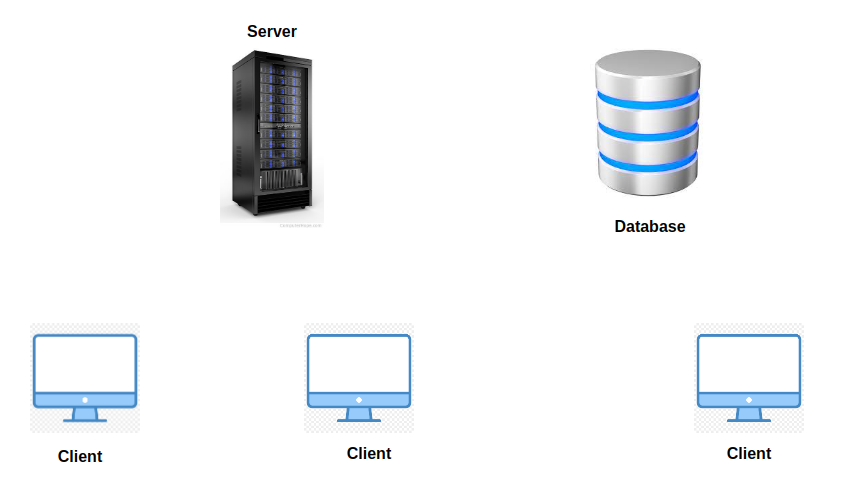
\includegraphics[width=10cm]{dfd-0.png}
    \caption{System Architecture}
    \label{fig:galaxy}
\end{figure}
The application is divided into the following components:
\begin{itemize}
    \item Server
    \item Client
    \item Database
\end{itemize}
There can be any number of clients in our system and all of the clients will run an instance of 'Client' separately from different machines. 

The clients cannot communicate with each other directly. 
The clients send messages to the server and server sends responses to that client and sometimes server has to send broadcast messages to every client. 

The server maintains a database so that it can handle all of the concurrency issues and sync all of the clients. 
Here we've used NoSql database so that Server can insert fields as per requirements.

\subsection{Data Flow}

\begin{figure}[htp]
    \centering
    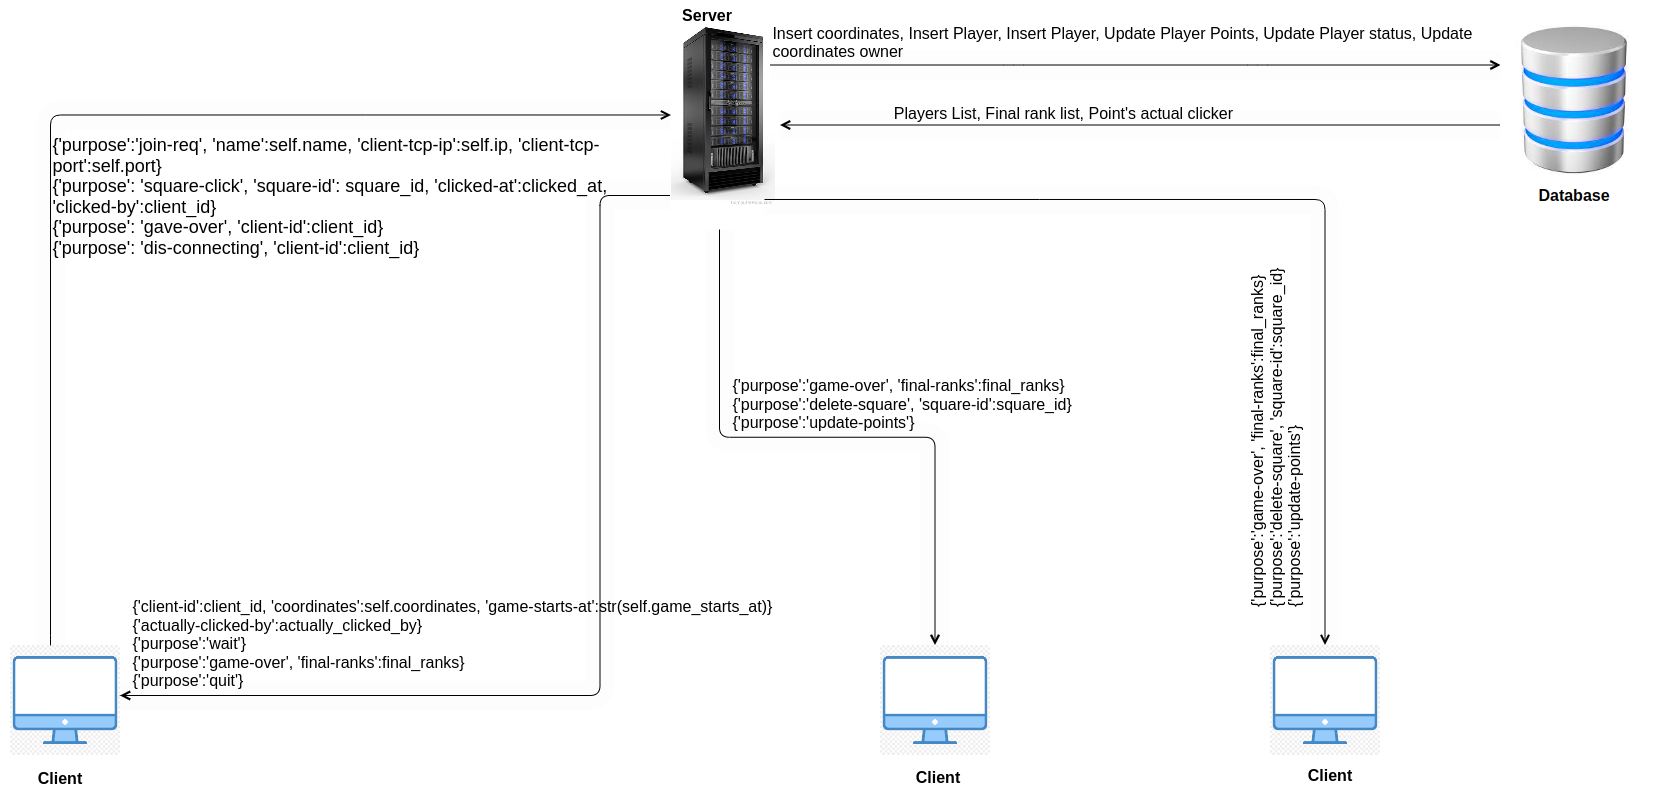
\includegraphics[width=15cm]{dataflow.png}
    \caption{Data flow}
    \label{fig:galaxy}
\end{figure}

\subsubsection{Messages from Client to Server}
\begin{itemize}
    \item {'purpose':'join-req', 'name':self.name, 'client-tcp-ip':self.ip, 'client-tcp-port':self.port}
    \item {'purpose': 'square-click', 'square-id': square\_id, 'clicked-at':clicked\_at, 'clicked-by':client\_id}
    \item {'purpose': 'gave-over', 'client-id':client\_id}
    \item {'purpose': 'dis-connecting', 'client-id':client\_id} 
\end{itemize}

\subsubsection{Messages from Server to a particular Client}
\begin{itemize}
    \item {'client-id':client\_id, 'coordinates':self.coordinates, 'game-starts-at':str(self.game\_starts\_at)}
    \item {'actually-clicked-by':actually\_clicked\_by}
    \item {'purpose':'wait'}
    \item {'purpose':'game-over', 'final-ranks':final\_ranks}
    \item {'purpose':'quit'}
\end{itemize}

\newpage
\section{Internal Modules}
There are mainly 5 internal modules in the application:
\begin{figure}[htp]
    \centering
    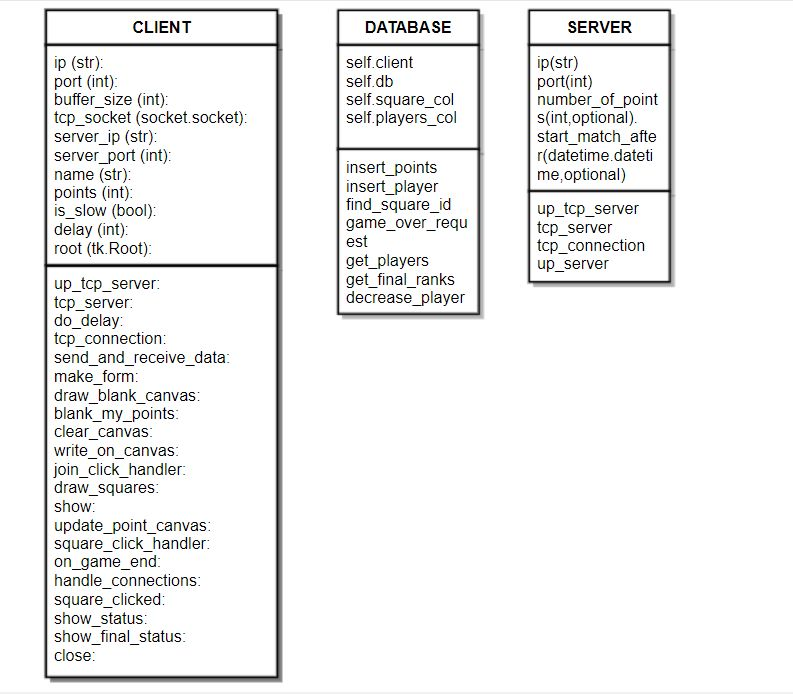
\includegraphics[width=10cm]{class-diagrams.jpeg}
    \caption{Classes}
\end{figure}

\textbf{Client} is the class. Each player has to run one instance of the \textbf{Client}.

\textbf{Server} is another class. Server machine will run one instance of the server.

\textbf{Database} is another class. Server maintains a database to handle concurrency issues and roll backing instructions for clients.

\textbf{Shared Module}: The shared module is used by both server and clients.

\subsection{server.py}
In the server there are a tcp server running always. The clients to that tcp server and sends the joining request. The server creates an record on the database for that client and sends an unique id for that client and the position of the co-ordinates of the squares as response. Also when the client send the input data, server stores the data and checks if some other player has clicked on that square previously, if yes then after matching the timestamps the server sends appropriate messages to both of the clients whether the points increases by the clients for themselves has to be decreased or not.

\subsection{client.py}
The client takes the ip address of server's tcp server and sends an joining request on the beginning. After server sends the response, client stores gets its id and waits for the starting time. When the starting time comes the client draws the squares on the screen.
When player clicks on a square, client first increase its points, then client sends that square id and timestamp when the square is clicked to the server. After the analyzing the timestamp if server sends to decrease the points, client decreases its points. 
Also, client listens to a different tcp server, and there can server sends a 'decrease-points' message, then also client decreases its points.

\subsection{database.py}

\subsection{measurements.py}
This is a shared module. Using the measurements module the server generates the points. Server uses the screen size, squares sizes to generate non-overlapping random points. Using this measurements and the coordinates the client makes its screen and draws the squares on the screen.

\section{Simulating Latency and Rolling back}

\subsection{Simulating Latency}
At the starting of client, it takes input whether the client is on a slow network. If it is entered yes, then after sending the request the client waits 'delay' amount of time also after getting the response the client waits also 'delay' amount of time before processing the delay. 
This delay actually simulates the delay in the network. Here we are physically simulating some amount of delay but in case of real network this delay will induced by the networks.

\subsection{Rollback}
\begin{figure}[htp]
    \centering
    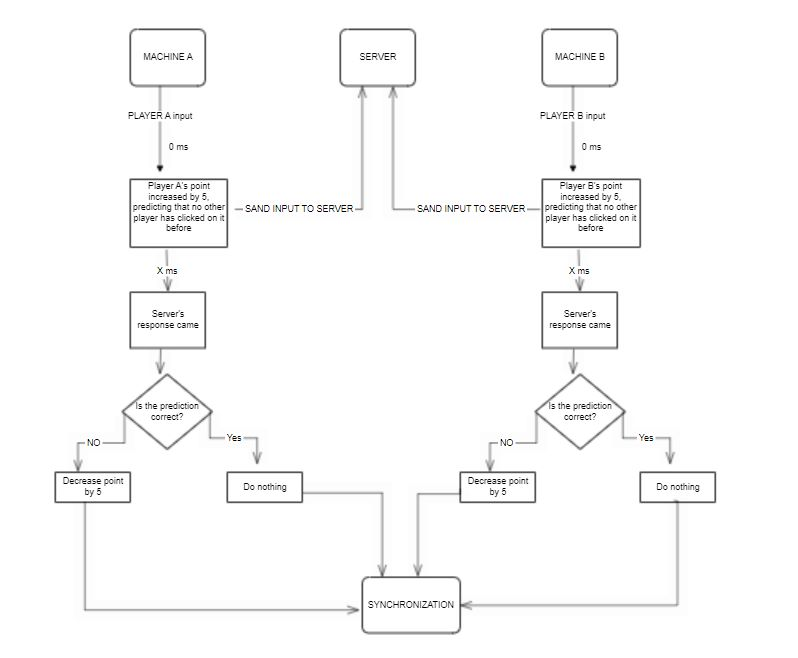
\includegraphics[width=10cm]{rollback.jpeg}
    \caption{Rollback}
    \label{fig:galaxy}
\end{figure}
Also please note that the client also has a tcp server to which server can send 'decrease-points' request. The reason is, lets assume a player A has clicked on square 5 on time t=10 but the request has reached to the server very late, say at t=50. Now assume that player B has clicked on the square 5 on time t=15 and this request has reached to the server at t=20 and server stored player B as winner for square 5. But when playerA's request has reached to server, the server has to tell player B to roll back, i.e. to decrease its points by 5. Now this request from server to client will go to the cilent's tcp server. And thus consistency will be held. And also server will make the clients wait until 'game-over' request (which indicates that game is over from all clients) came from all clients. 

\section{External Modules}
Several external modules are used in the application:
\begin{itemize}
\item {\verb|tkinter|}: Tkinter is used to make the GUI 
\item {\verb|sphinx|}: Sphinx is used to make project documentation
\item{\verb|pymongo|}: Pymongo is used to connect database and server.
\item{\verb|datetime|}: To get timestamps for clicking times.
\item{\verb|socket|}: To do the networking stuffs the socket python library is used.
\end{itemize}

\section{Screenshots of GUI}
\begin{figure}[htp]
    \centering
    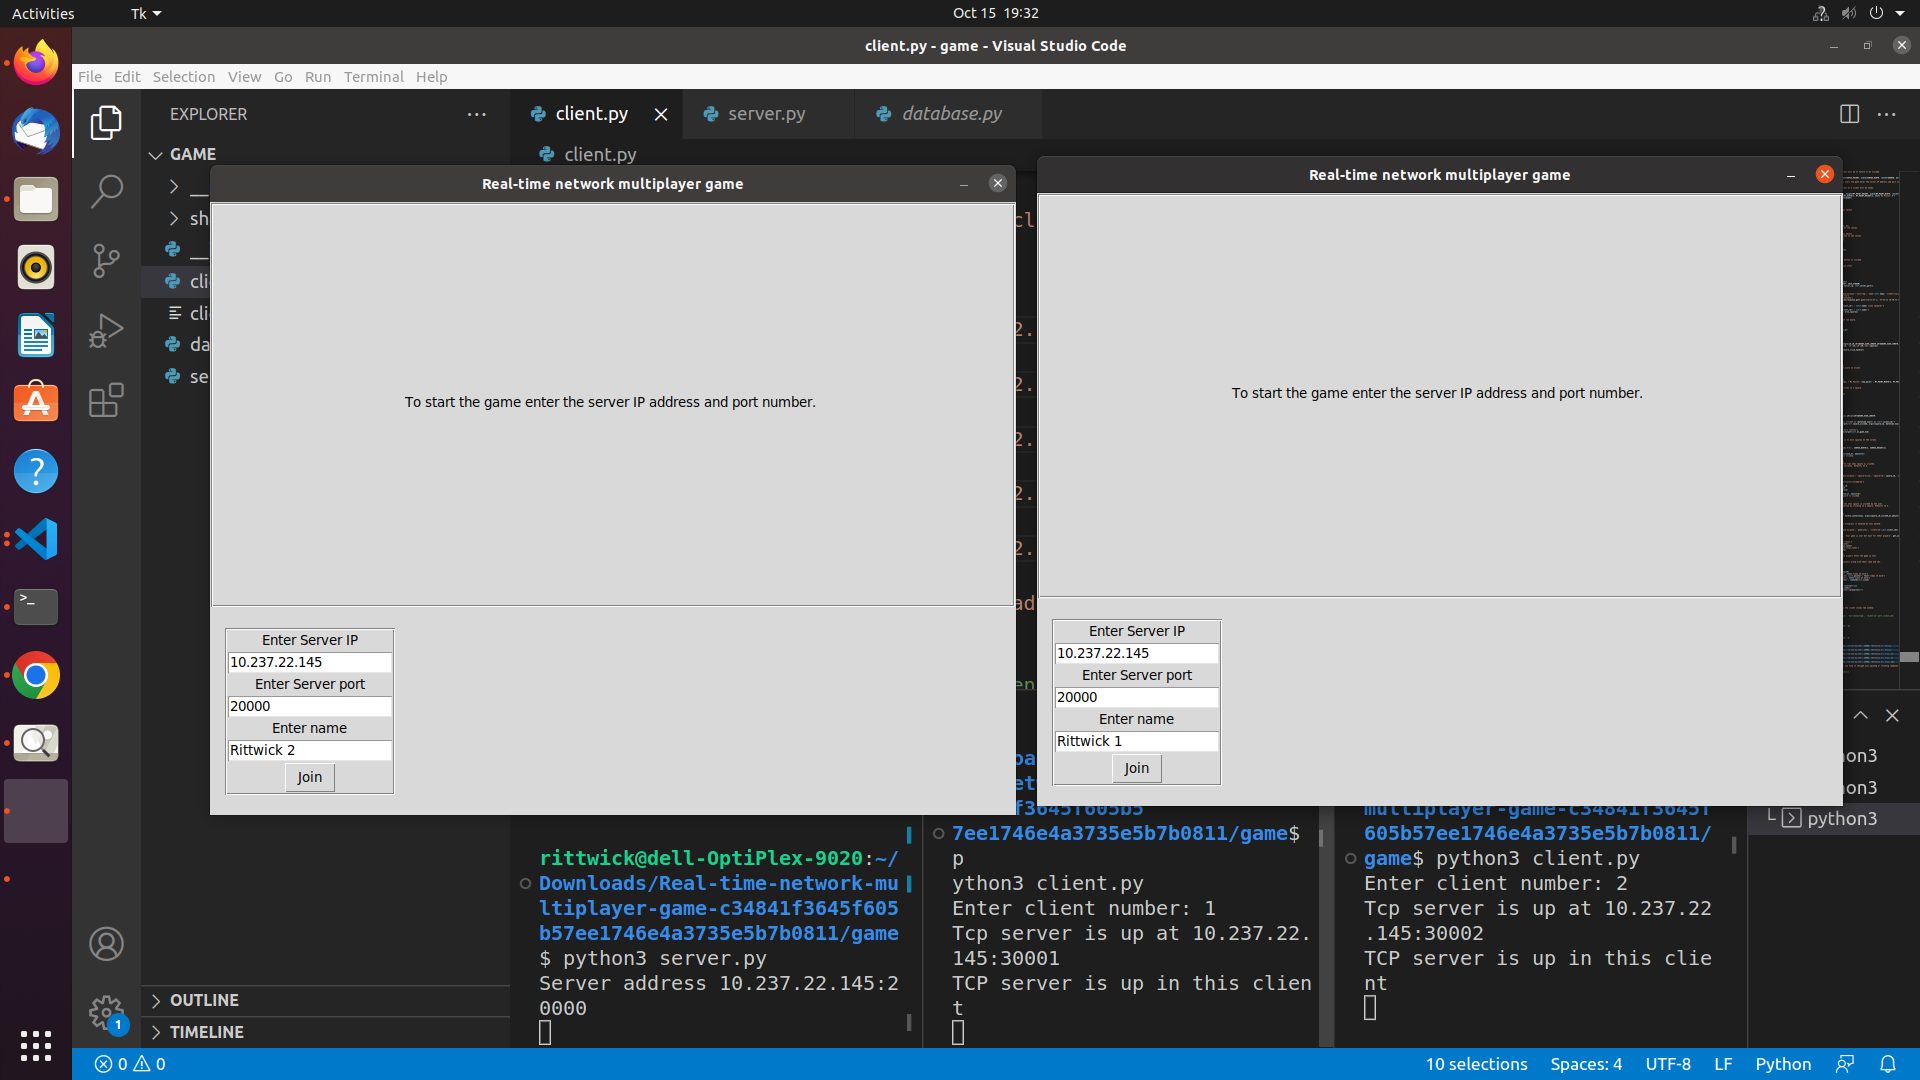
\includegraphics[width=10cm]{1.png}
    \caption{Joining Screen}
    \label{fig:galaxy}
\end{figure}
\begin{figure}[htp]
    \centering
    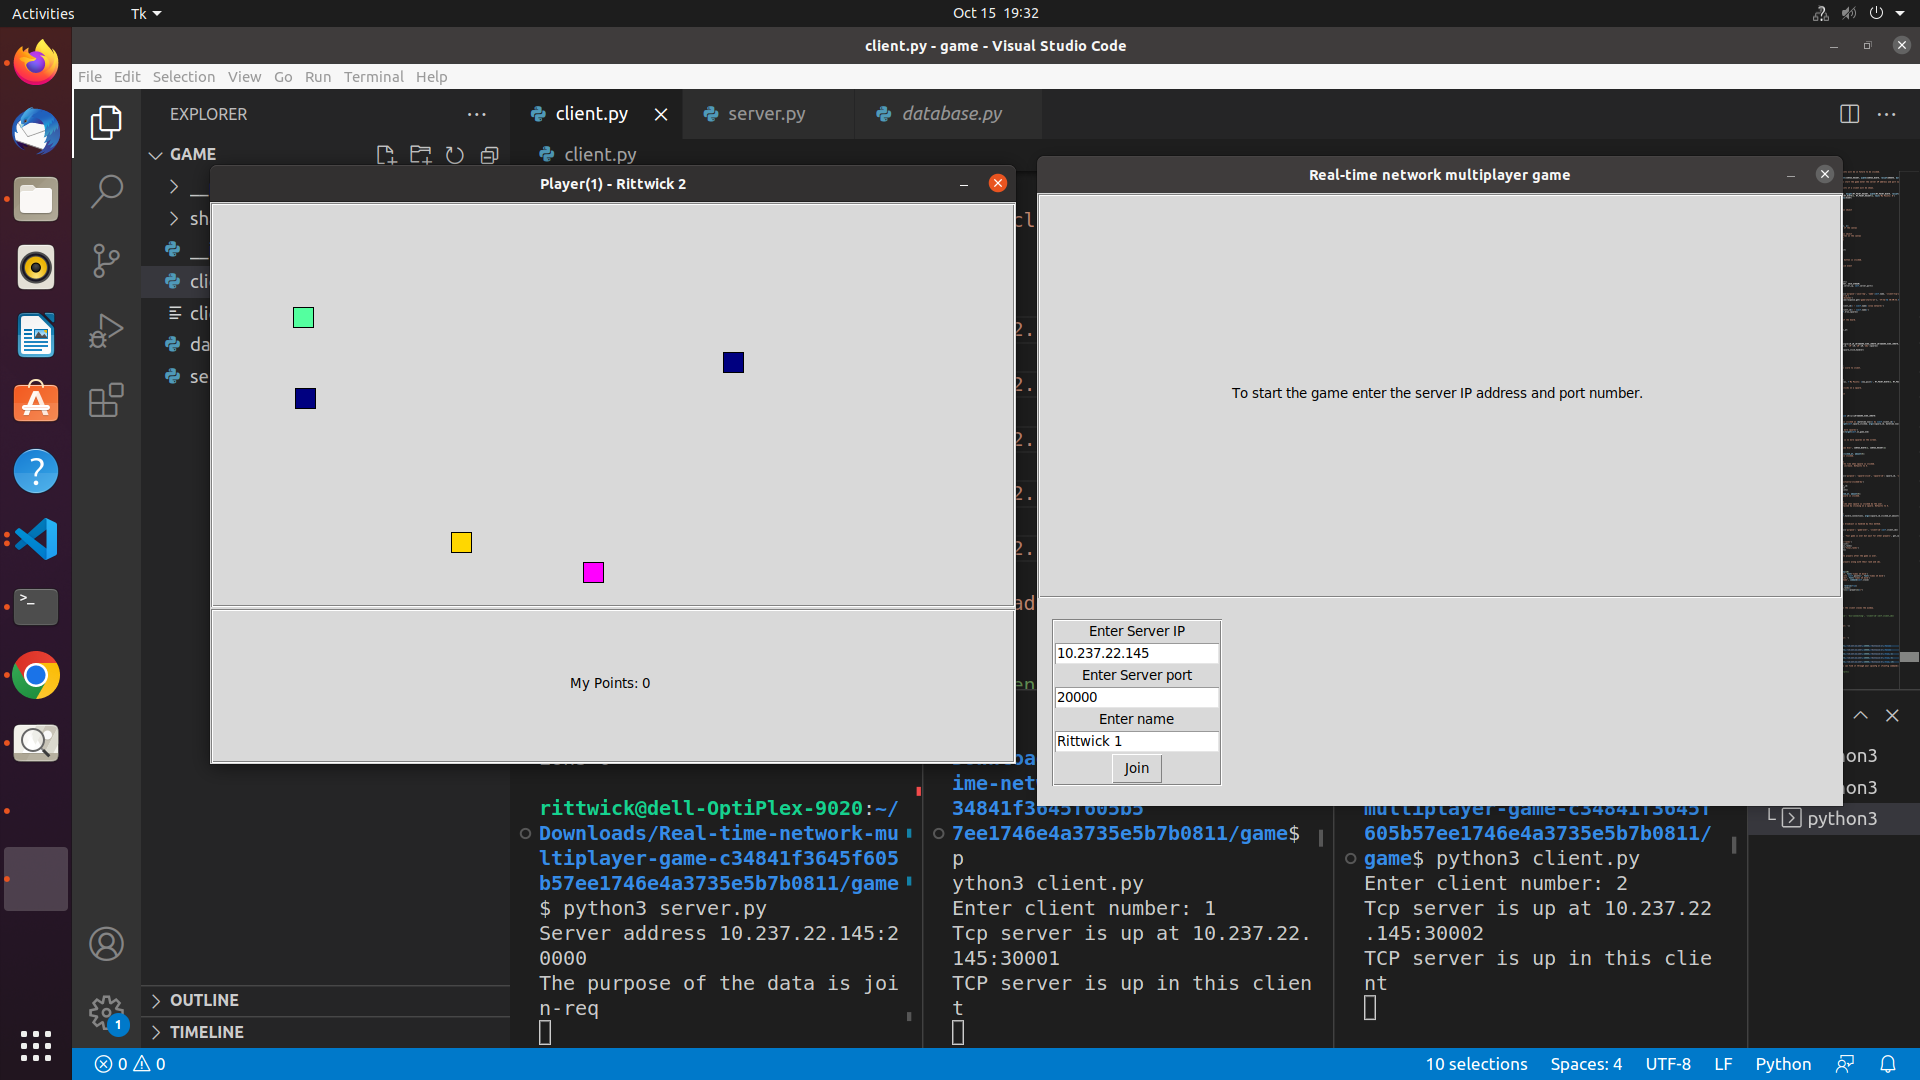
\includegraphics[width=10cm]{2.png}
    \caption{}
    \label{fig:galaxy}
\end{figure}
\begin{figure}[htp]
    \centering
    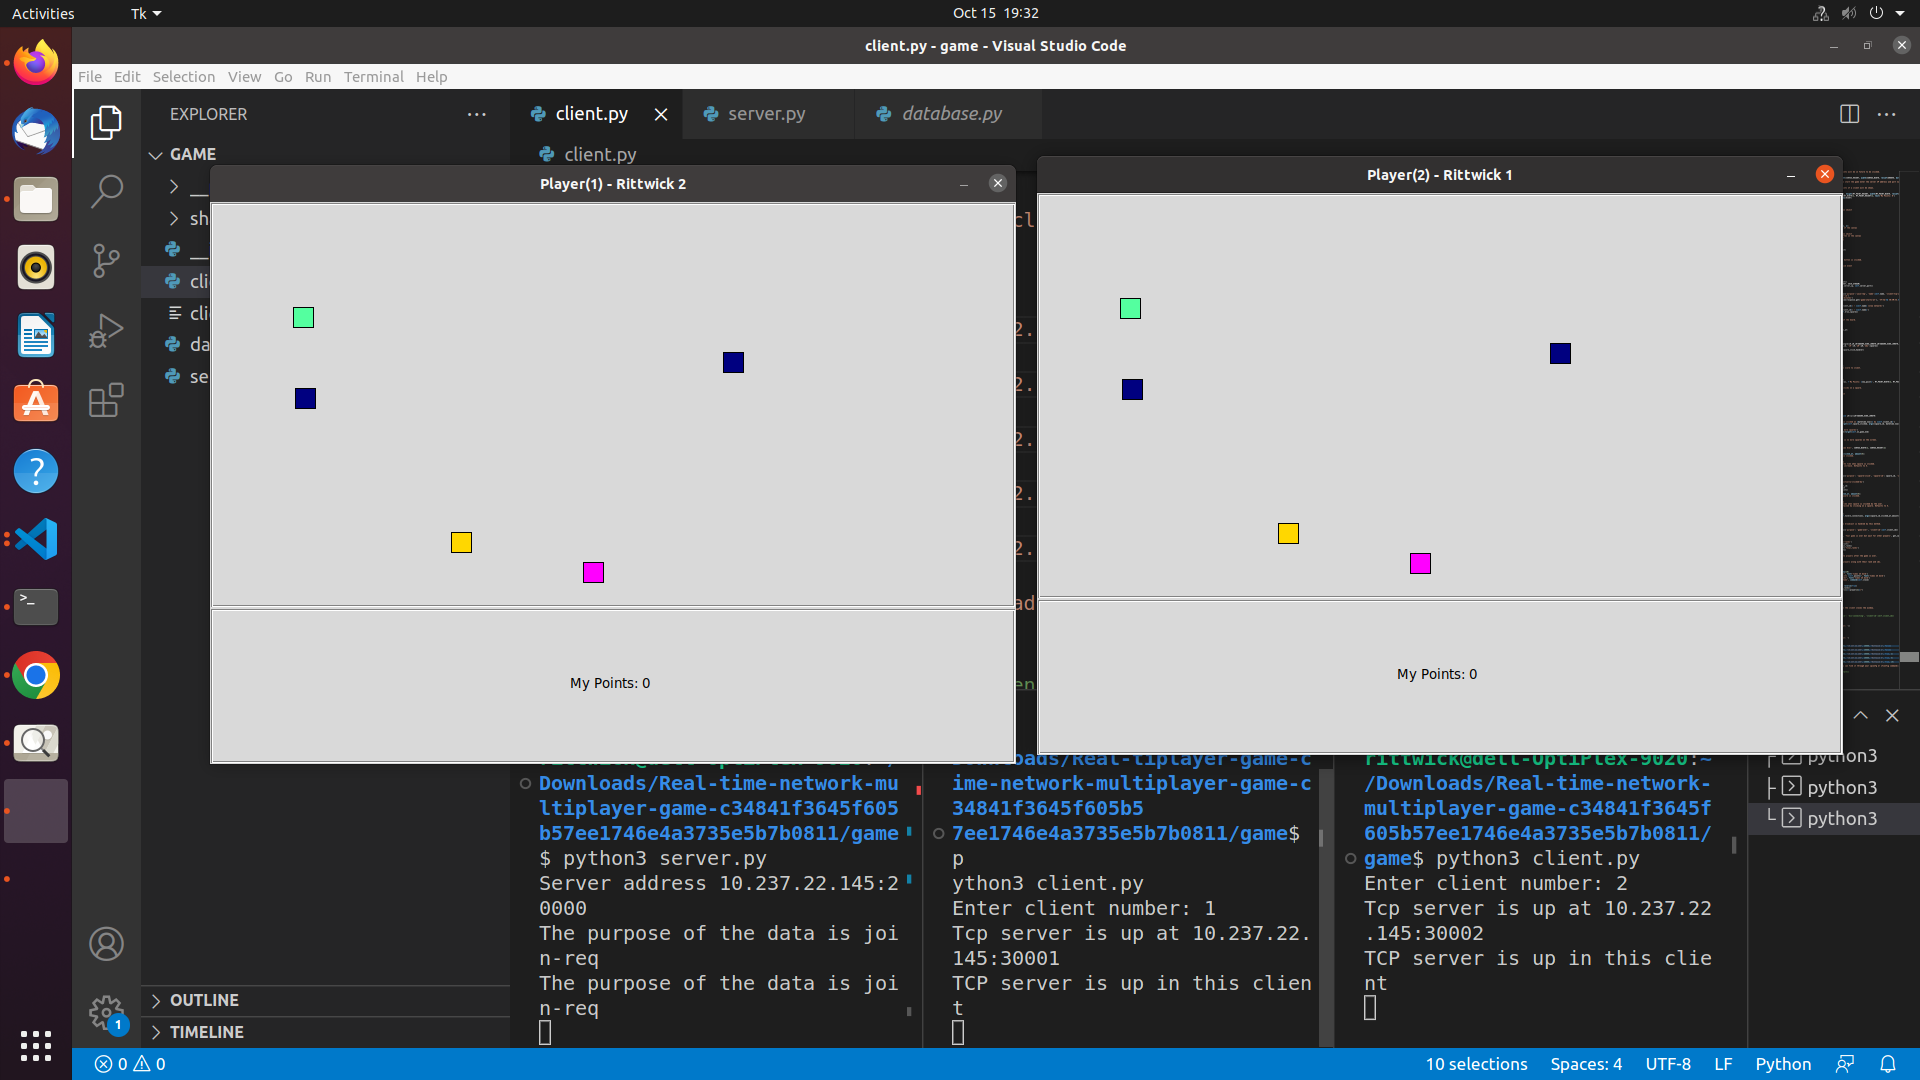
\includegraphics[width=10cm]{3.png}
    \caption{After the points are rendered on the screen.}
    \label{fig:galaxy}
\end{figure}
\begin{figure}[htp]
    \centering
    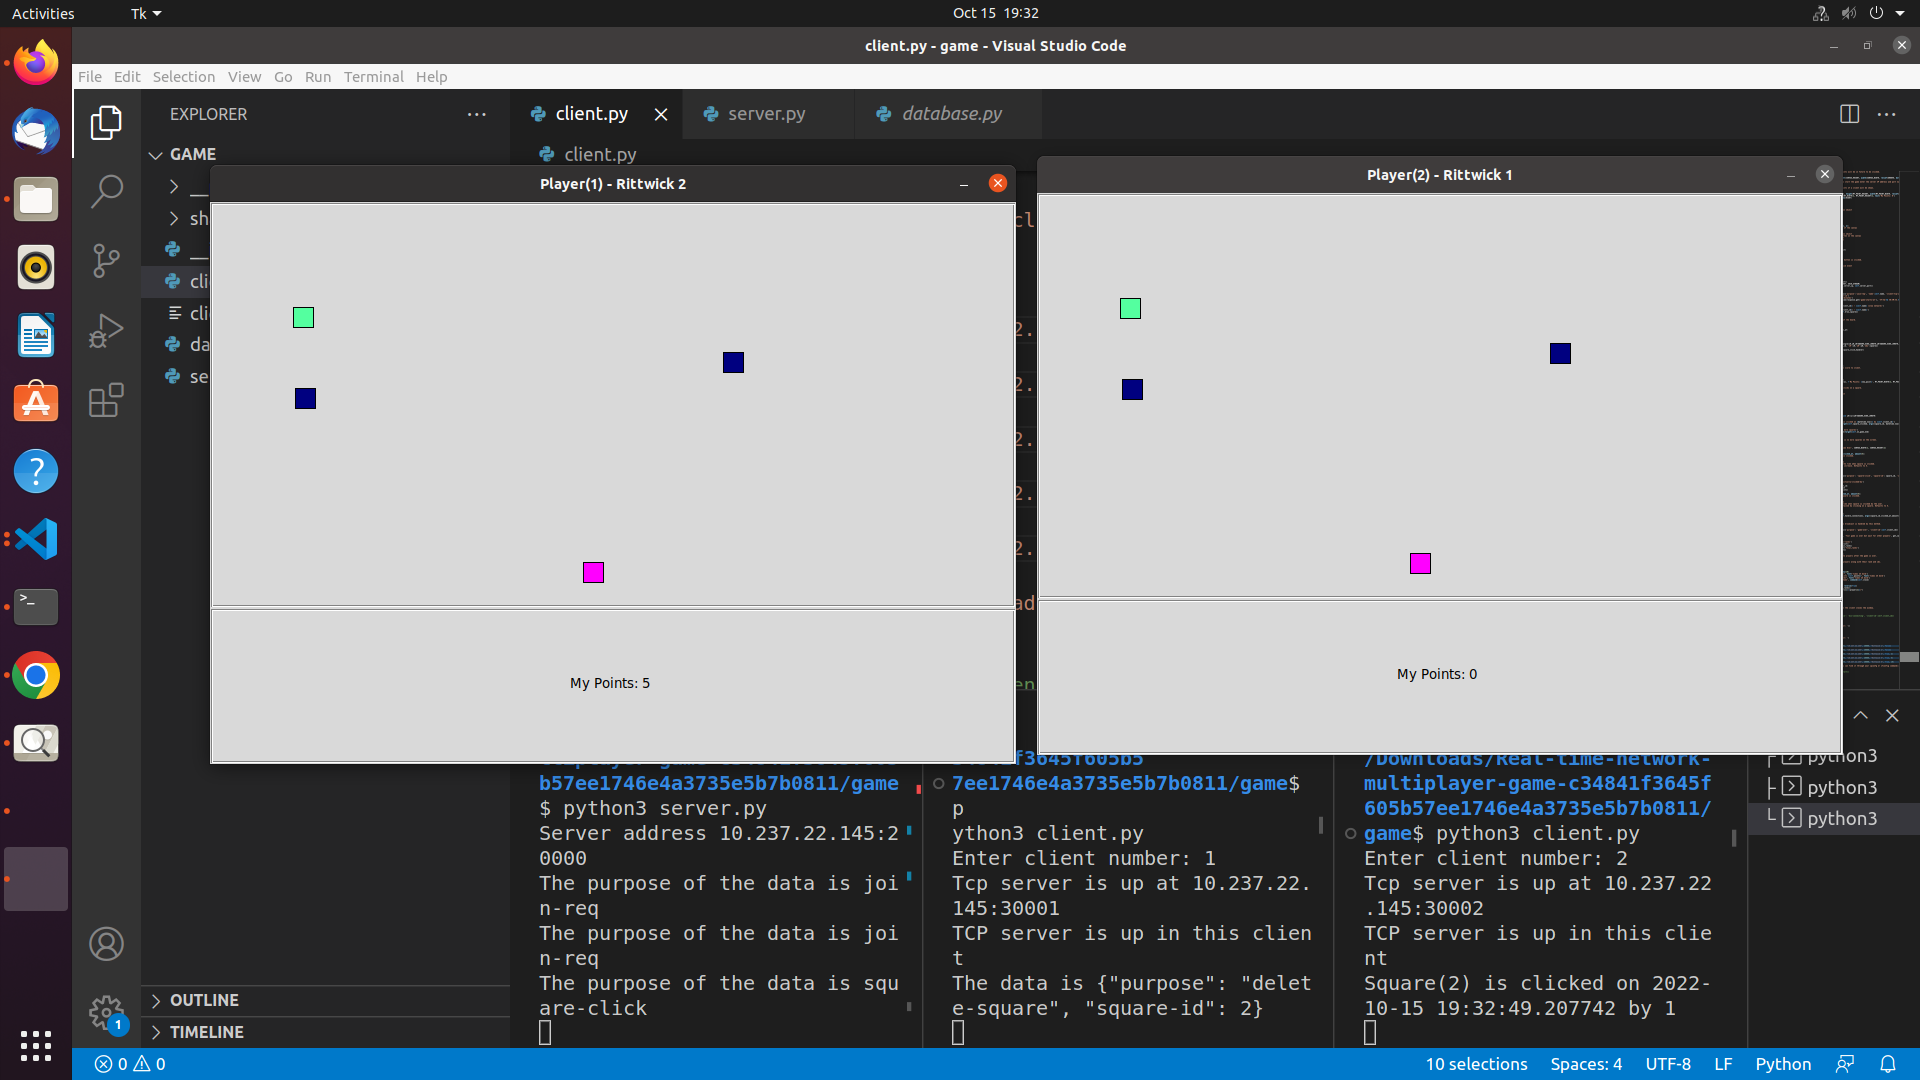
\includegraphics[width=10cm]{4.png}
    \caption{}
    \label{fig:galaxy}
\end{figure}
\begin{figure}[htp]
    \centering
    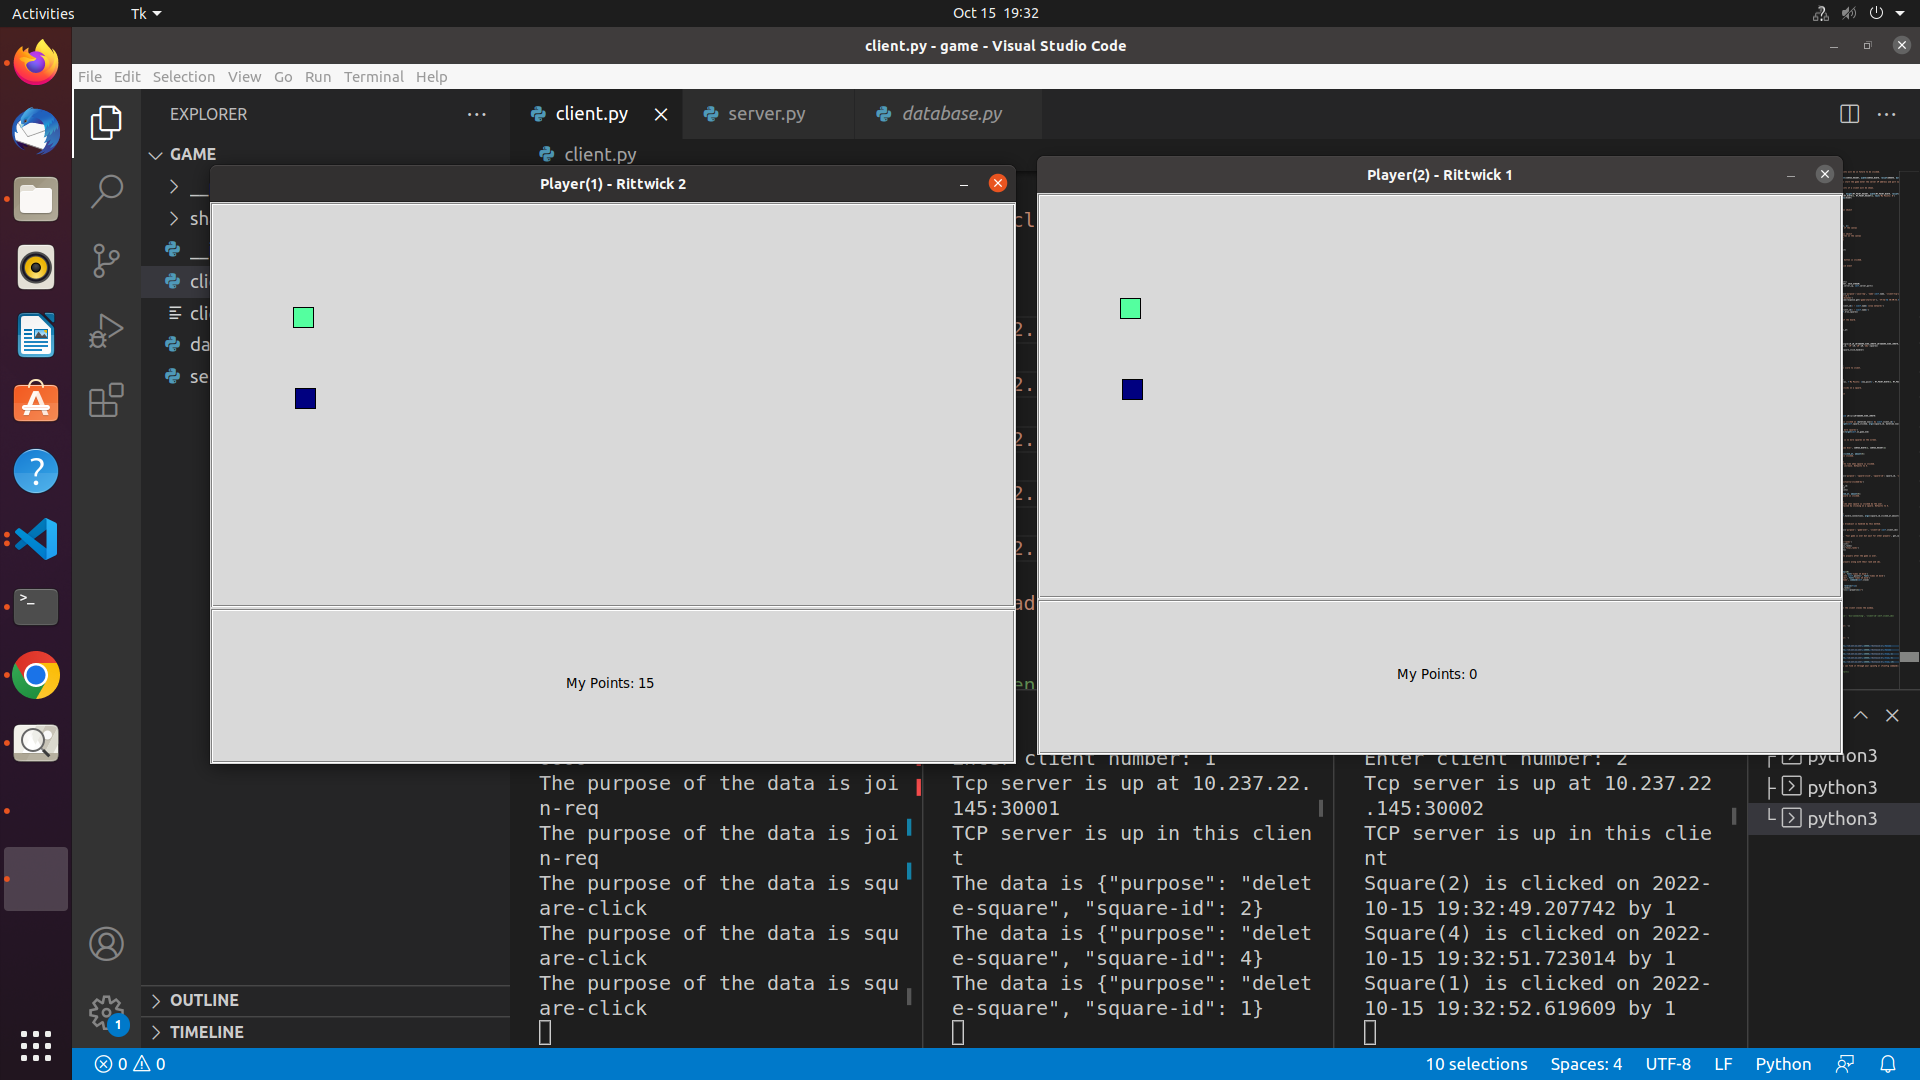
\includegraphics[width=10cm]{5.png}
    \caption{}
    \label{fig:galaxy}
\end{figure}

\begin{figure}[htp]
    \centering
    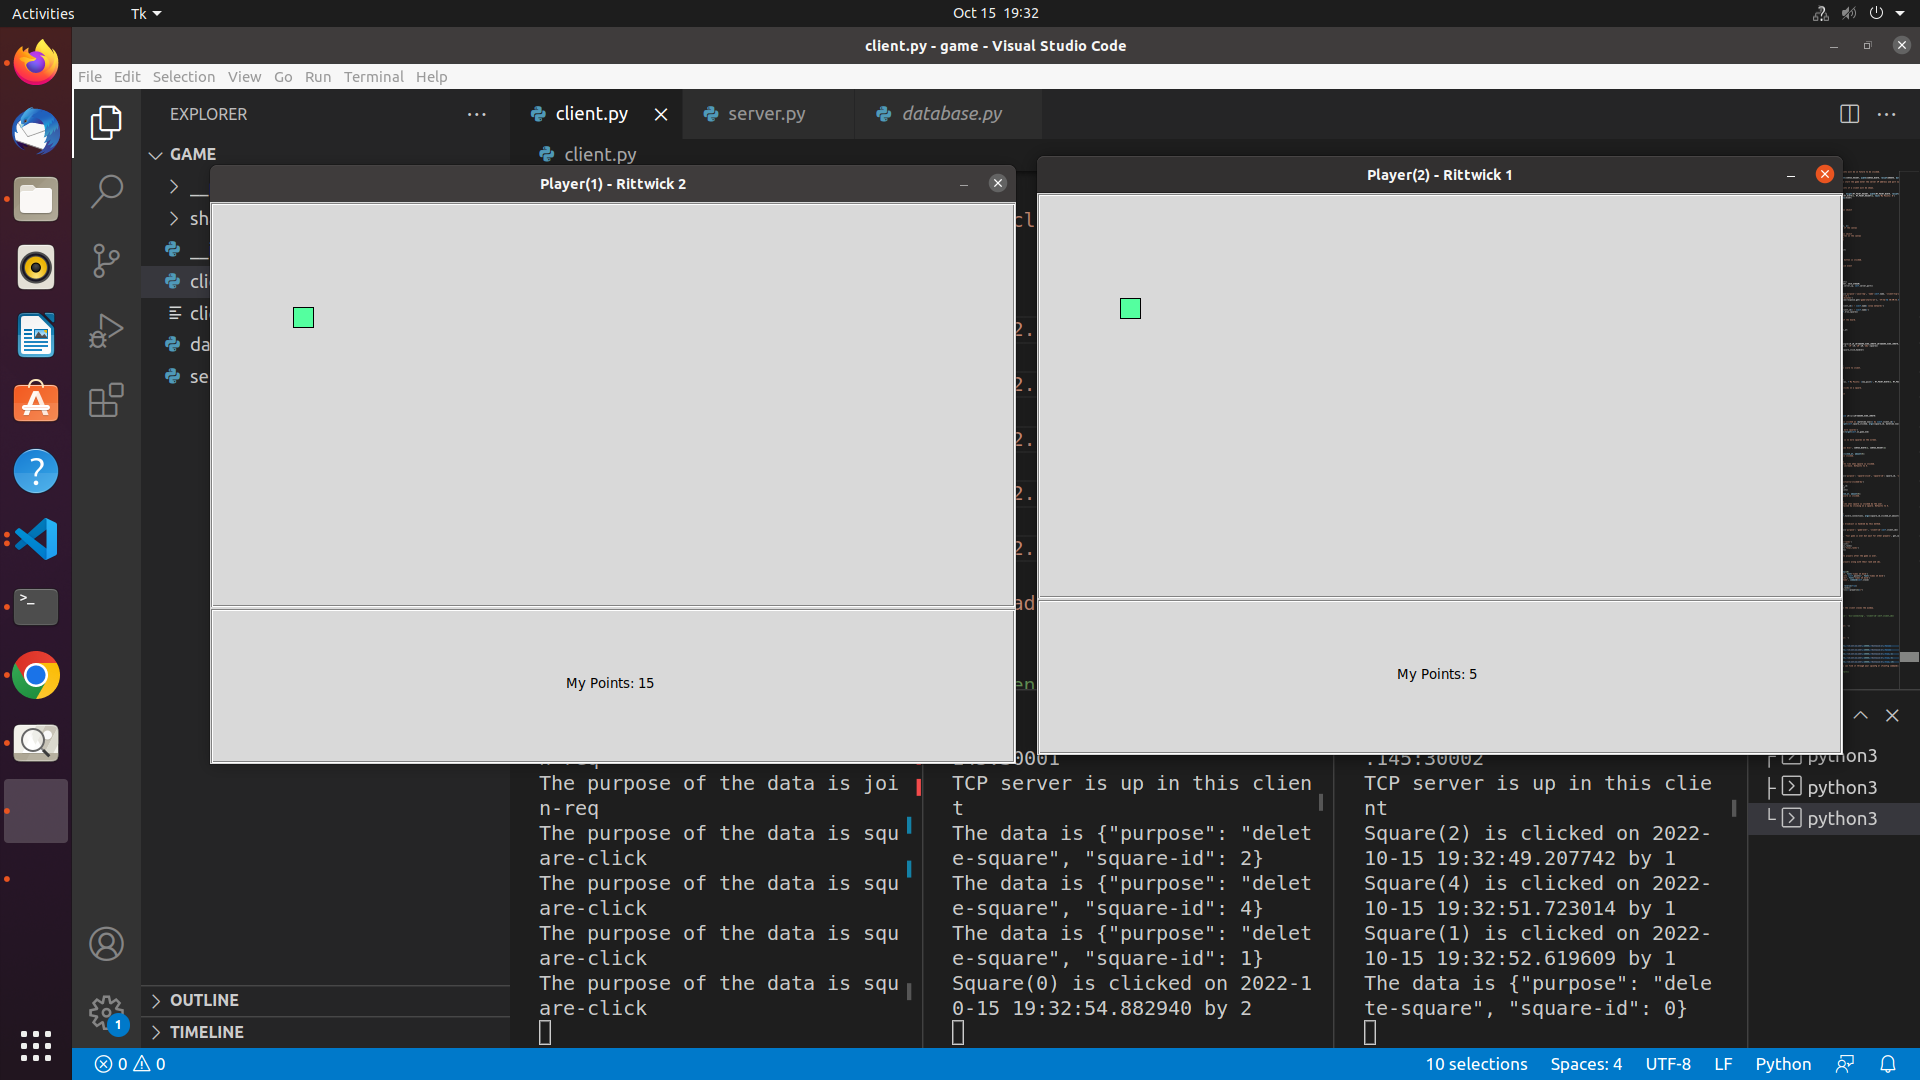
\includegraphics[width=10cm]{6.png}
    \caption{}
    \label{fig:galaxy}
\end{figure}\begin{figure}[htp]
    \centering
    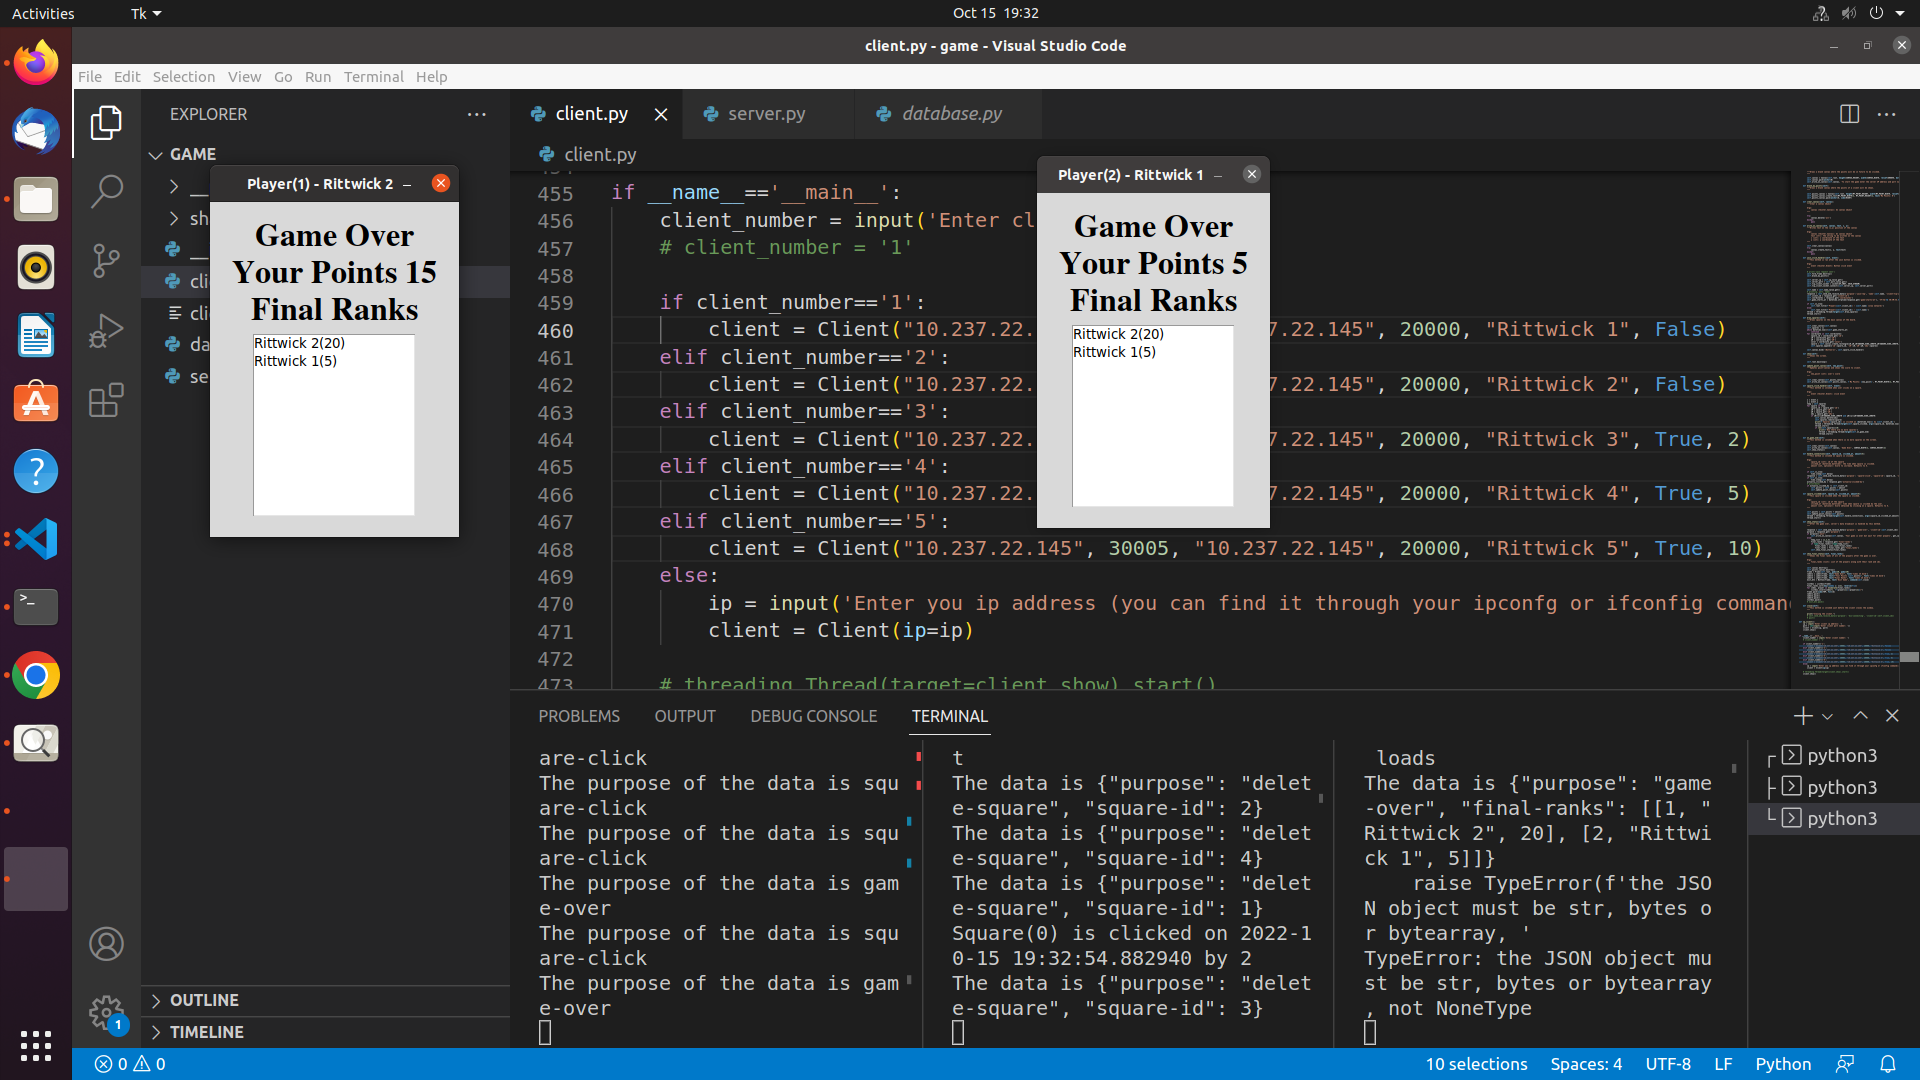
\includegraphics[width=10cm]{7.png}
    \caption{}
    \label{fig:galaxy}
\end{figure}

\vfill
\clearpage
\section{}
\begin{itemize}
    \item Version Control Using github.com. The link to git repository: \href{https://github.com/rittwickBhabak/Real-time-network-multiplayer-game/tree/main}{https://github.com/rittwickBhabak/Real-time-network-multiplayer-game/tree/main}
    \item Project documentation using Sphinx Library
    \item Redistribute package, whl file
\end{itemize}

\section{Further Scope}
\begin{itemize}
    \item Presently the project has been developed taking one time zone into consideration i.e. Indian local time. The same may be expanded to client working in different geographic location with different time zone. For ex. Different client in India and US.
\end{itemize}

\section{Contribution by Different Group Members}
\begin{itemize}
    \item {\verb|Rittwick Bhabak|}: Contributed in deciding the architecture and has build the server module and client module. (50\% of total contribution)
    \item {\verb|Sagar Agrawal|}: Contributed in deciding the architecture and build some parts of database module and made the project documentation. (25\% of total contribution)
    \item {\verb|Manik Jain|}: Contributed in deciding the architecture and build some parts of database modules and shared module and made the automated documentation of the project. (25\% of total contribution)
\end{itemize}

\printbibliography

\begin{acks}
We would like to express our special thanks of gratitude to my teacher Rahul Narain sir as well as our TA and CodeWithHarry\cite{codewithharry} YouTube Channel, Codemy.com\cite{codemy} YouTube channel, AI Swiget\cite{atbswp} and Bhagath Mamindlapelly YouTube channel who helped us to do this wonderful project on the topic \textbf{Real-time network multiplayer game}, as a result we learnt so many new things. We are really thankful to them.
\end{acks}

%%
%% If your work has an appendix, this is the place to put it.
\appendix

\end{document}
\endinput
%%